\section{Scan Window Processing}\label{sec:haar}

\fixme{Sharmila holds the lock}


Once the classifiers are obtained, the next step is to apply these classifiers to detect faces in the image. 

Specification of classifiers:
Each Haar classifier has up to 3 rectangles and has a fixed size of 25x25 as shown in Figure~\ref{fig:classifier}. 
Several weak Haar Classifiers are combined in weighted sum to form Strong Classifiers. 
Our algorithm consists of 25 stages of strong classifiers with a total of 2913 Haar classifiers. 
The information about the classifiers is completely provided by x,y coordinates of the starting 
pixel of a rectangle in Haar classifier, width, height, weight of each rectangle, threshold for 
Haar classifier and threshold for each stage. 
\begin{figure}[h]
  \centering 
  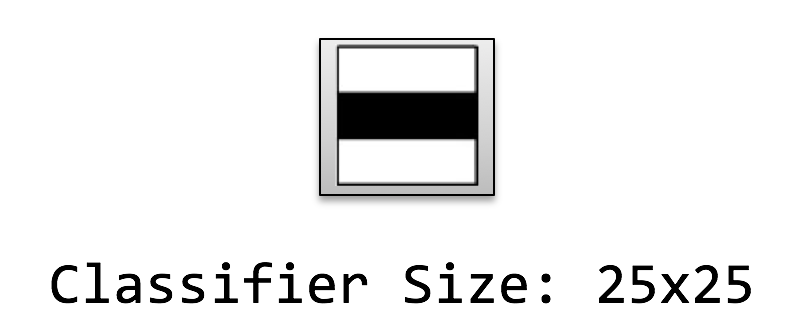
\includegraphics[width=\linewidth]{figs/classifier.jpg}
  \caption{Example of Classifier with three rectangles \textnormal{\small }  }
  \label{fig:classifier}
\end{figure}


Overview of scan window processing:
For a given image, we consider a scan window of size 25 x 25 starting from the top left corner. 
The scan window is identified by x,y coordinates of its starting pixel. Each scan window is 
then passed through the stages of strong classifiers to detect if they contain the haar features. 

Each Haar classifier of Stage i contains up to three rectangles. The rectangle is defined by 
x,y coordinates of its starting pixel, its width and height. This data is used to calculate the 
four corners of the region in scan window corresponding to this rectangle. Then, we use the 
integral image to calculate the sum of the pixels of the rectangle’s region. Each Haar rectangle
is also associated with a weight that is used to calculate the weighted sum of the scan window for Haar
classifier. The accumulated sum is determined for all the Haar classifiers in Stage i. If the sum 
is greater than threshold[i], the scan window is considered to pass Stage i.

The scan window that passes through all the stages is considered to be a face. 
The next scan window is chosen by incrementing the pixel number. The process is repeated for all 
the scan windows of the image. As an example, for a 1024 x 1024 image, there are 1000 x 1000 = 106 
scan windows (excluding the right and bottom 24 pixels) as shown in Figure~\ref{fig:img_scan}. 
\begin{figure}[h]
  \centering 
  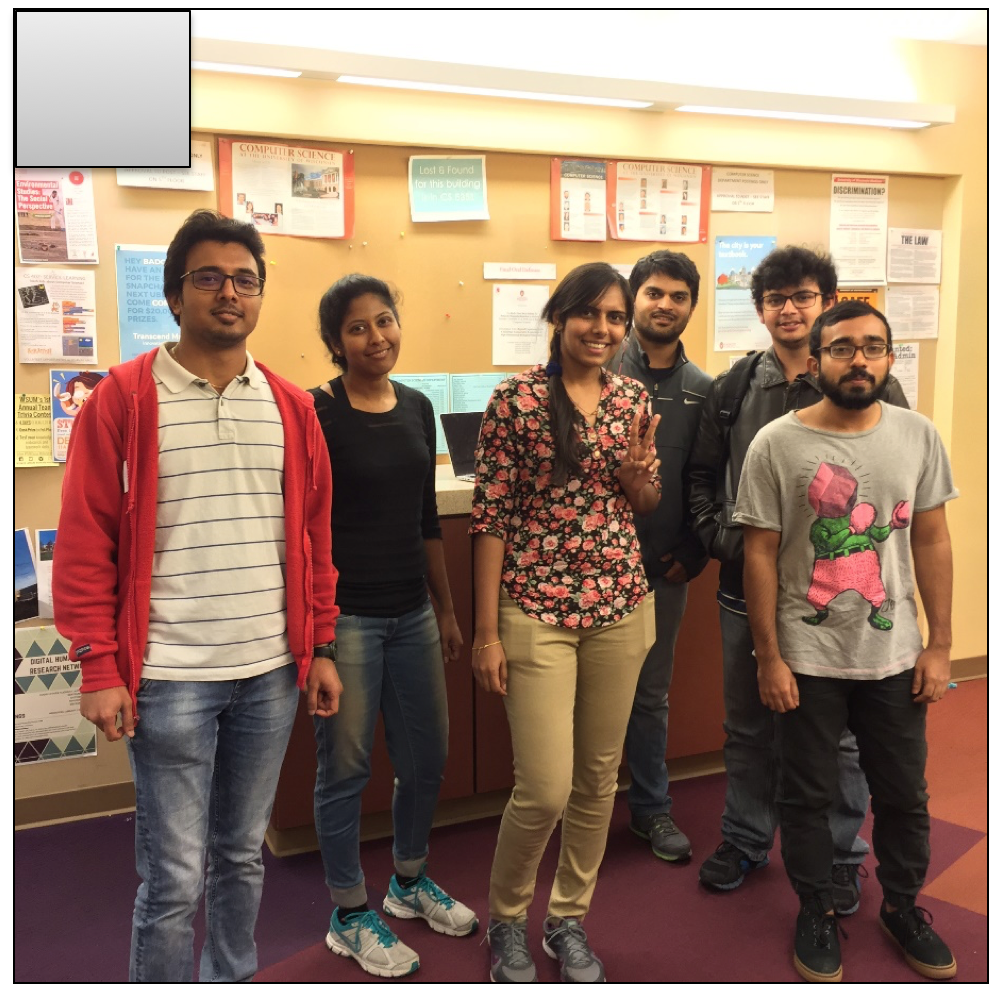
\includegraphics[width=\linewidth]{figs/img_with_scan.jpg}
  \caption{An image with scan window \textnormal{\small }  }
  \label{fig:img_scan}
\end{figure}


Baseline implementation:
As seen in the overview, each scan window is processed independently. Hence one thread is assigned 
to process a scan window. For 1024x1024 image, we require 10^6 threads. Hence there is a huge scope 
for parallelism. Each scan window is processed through all 25 stages to detect a face. 

Bit Vector:
We keep a bit vector to keep track of rejected scan windows. The bit vector is set true initially 
and copied to device memory  of GPU. If a scan window is rejected at any stage, the bit corresponding 
to this scan window is set false.  If a bit in BV is true at the end of the scan window processing, 
the scan window is considered to have face.  After the processing of all the scan windows, 
the bit vector is copied back to Host Memory. From this bit vector,  on host, we identify the
starting address of scan windows that contain faces and push the coordinates to vector. 


